% The idea is to use a shared feature space for all tasks, while each task also has a separate layer for making the prediction.
\begin{abstract}
	Hard parameter sharing for multi-task learning is widely used in empirical research despite the fact that their generalization properties have not been well established in many cases. This paper studies a fundamental question to better understand this approach: How does hard parameter sharing work given multiple linear regression tasks? We develop new techniques and establish a number of new results in the high-dimensional setting, where the sample size and feature dimension become increasingly large in a fixed ratio. First, we show a sharp bias-variance decomposition of hard parameter sharing, given multiple tasks with the same features. Second, we characterize the asymptotic bias-variance limit for two tasks, even when they have arbitrarily different sample size ratios and covariate shifts. We also demonstrate that these limiting estimates for the empirical loss are incredibly accurate in moderate dimensions. Finally, we explain an intriguing phenomenon where increasing one task's sample size helps another task initially by reducing the variance but hurts eventually due to the increasing bias. This suggests progressively adding data for optimizing hard parameter sharing, and we validate its efficiency in text classification tasks.
\end{abstract}

\section{Introduction}\label{sec_introduction}

Hard parameter sharing (HPS) for multi-task learning is widely used in empirical research and goes back to the seminal work of \citet{C97}.
Recent work has revived interest in this approach because it improves performance and reduces the cost of collecting labeled data \cite{MTDNN19,ZSSGM18}.
It is generally applied by sharing the feature layers between all tasks while keeping an output layer for every task.
Often, hard parameter sharing offers two critical advantages if successfully applied.
(i) It reduces model parameters since all tasks use the same feature space.
(ii) It reduces the amount of labeled data needed from each task by augmenting the entire training dataset.

Hard parameter sharing offers great intuitive appeal as an inductive transfer mechanism.
It reduces overfitting by acting as a regularizer \cite{R17}.
For example, by restricting the shared space's size, HPS encourages information sharing among multiple tasks \cite{KD12}.
Another source of inductive bias comes from the tasks and depends on datasets' properties such as sample sizes and task covariances \cite{WZR20}.
However, how these dataset properties impacts HPS has not been established.
%It becomes increasingly important to understand HPS' formal generalization properties.
Part of the challenge may be that HPS' generalization performance depends intricately on the sample size ratios and covariate shifts between tasks, not amenable to standard concentration results.
Previous results based on Rademacher complexity or VC dimensions have considered when all tasks' sample sizes are equal to logarithm factors of feature dimension \cite{B00,MPR16}, and when all tasks' sample sizes increase simultaneously \cite{AZ05,M06}.
%For, the generalization error scales down as the sample sizes of all tasks increase, when applied to the multi-task setting \cite{B00,AZ05,M06,MPR16,WZR20}.

\begin{figure*}[!t]
	\begin{subfigure}[t]{0.5\textwidth}
		\centering
		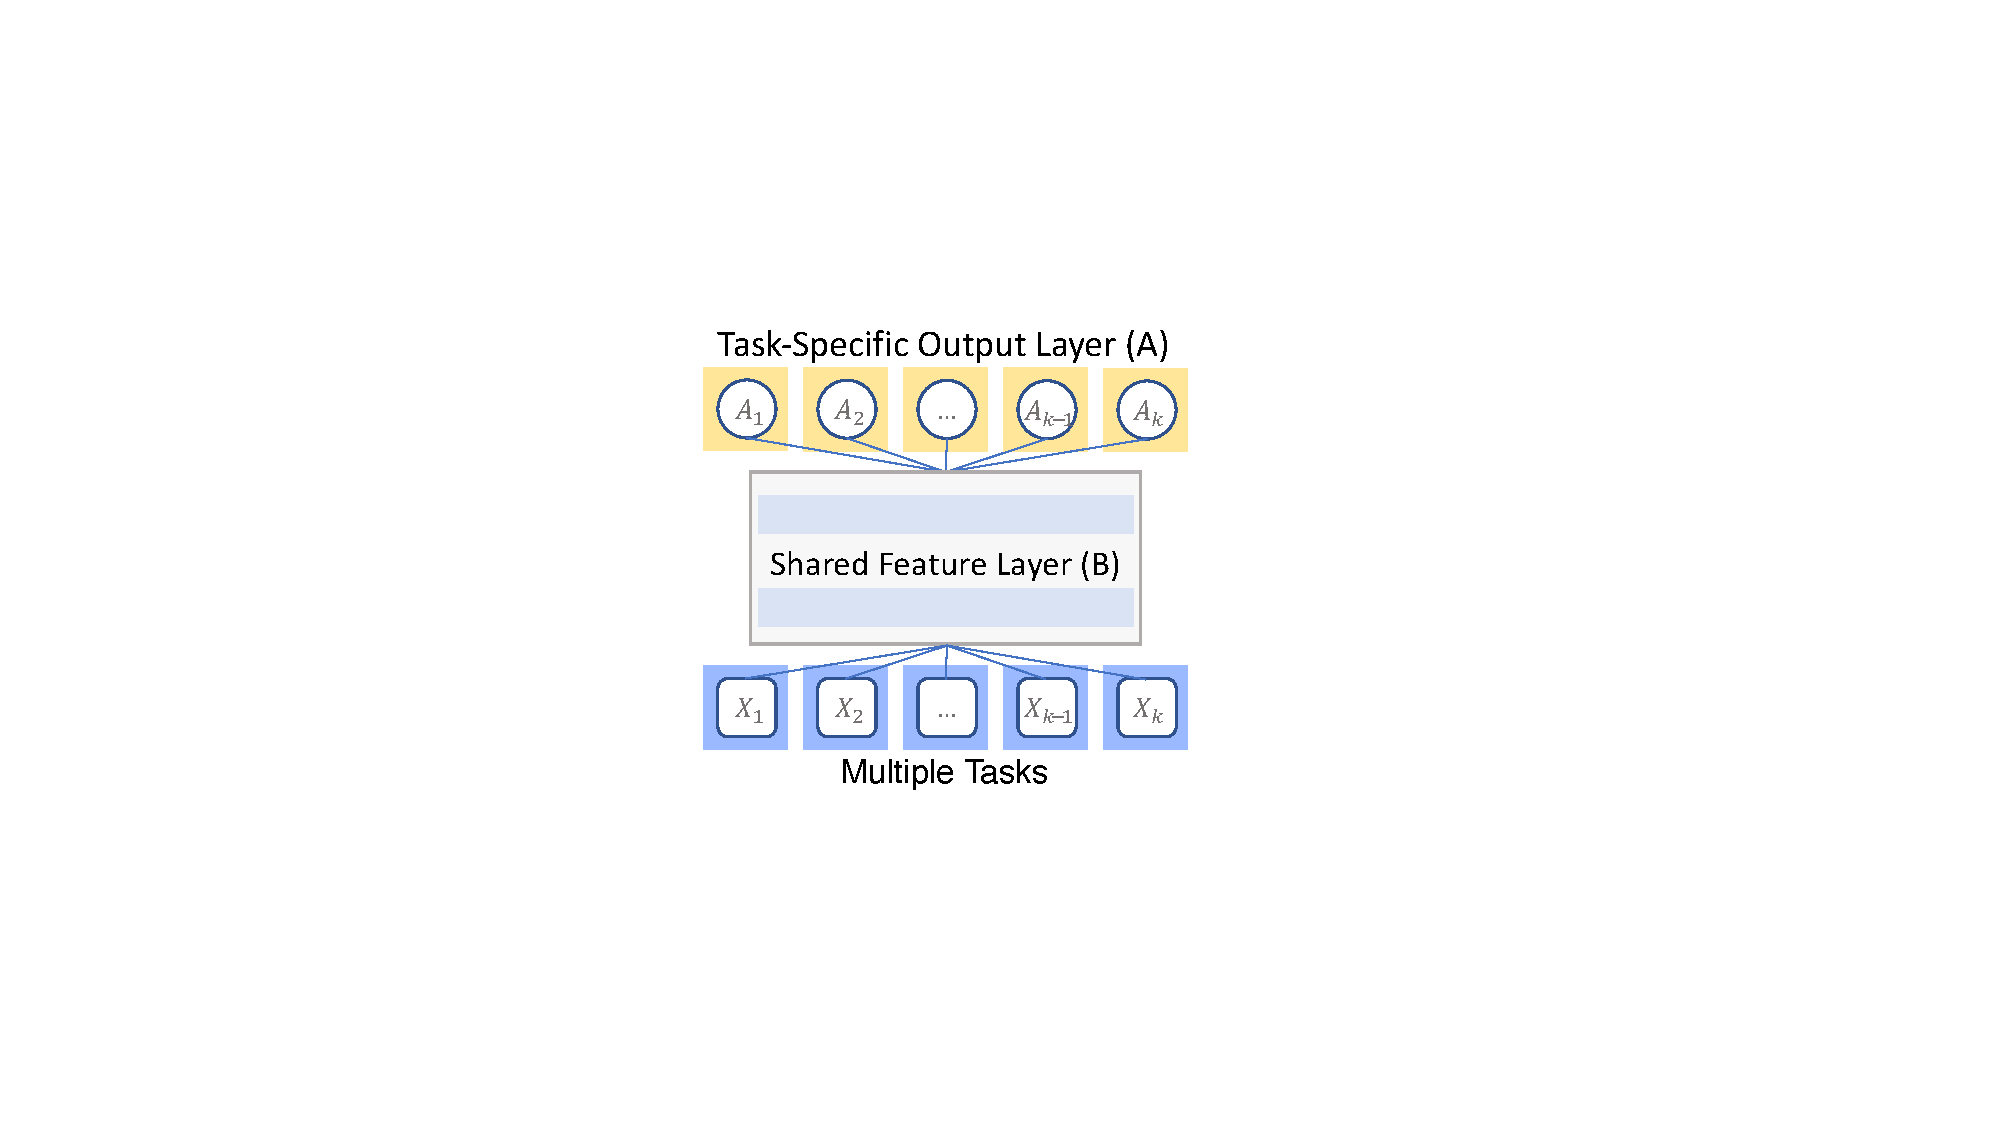
\includegraphics[width=0.5\textwidth,valign=t]{figures/mtl_model_arch.pdf}
		\caption{A hard parameter sharing architecture}
	\end{subfigure}\hfill
	\begin{subfigure}[t]{0.5\textwidth}
		\centering
		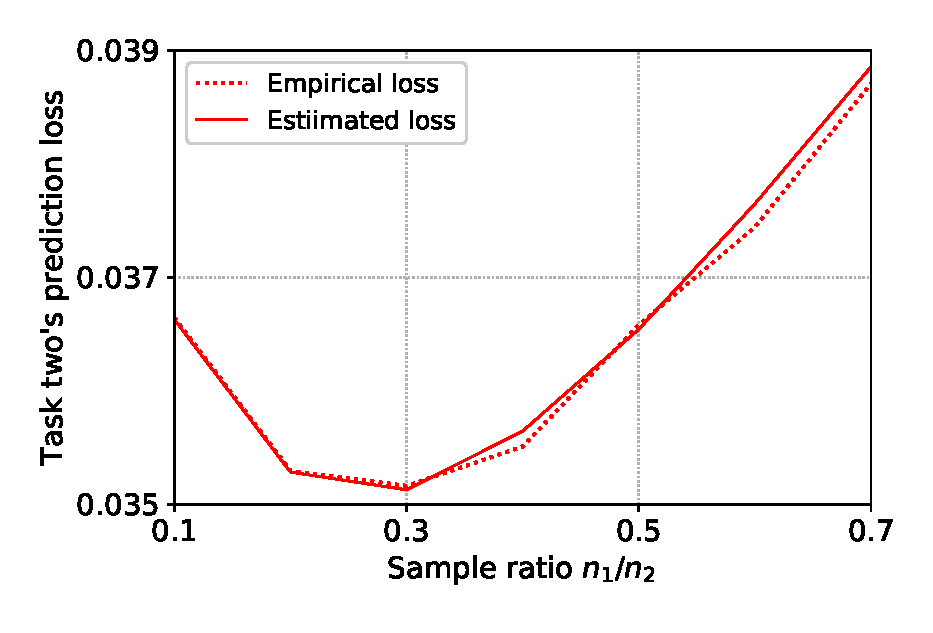
\includegraphics[width=0.713\textwidth,valign=t]{figures/sample_ratio_c2_400.eps}
		\caption{Varying sample size ratio}
		\label{fig_intro_sample_size_b}
	\end{subfigure}
	\caption{An illustrative example of our result:
	Consider the prediction loss of hard parameter sharing (left) for task two, given two linear regression tasks.
	Increasing task one's sample size decreases task two's prediction loss initially, but increases afterwards. This phenomenon occurs due to different bias-variance tradeoffs as the sample size ratio increases. Our result provides an estimated loss (solid line) that accurately matches the empirical loss (dotted line).
	See Section \ref{sec_simulation} for the precise setting.}
	\label{fig_intro_sample_size}
\end{figure*}



This paper presents new techniques to study hard parameter sharing and establish a number of new results.
We consider regression analysis, which is arguably one of the most fundamental problems in statistics and machine learning.
We are interested in the \textit{high-dimensional} setting, where each dataset's sample size and feature dimension grow linearly at a fixed ratio.
This is motivated by many multi-task learning applications, where the amount of labeled data from each dataset is usually insufficient for learning a single task.
For example, this is the case if a dataset's sample size is only a small constant factor of the feature dimension.
The high-dimensional setting is challenging but is crucial for understanding how datasets' sample sizes impact generalization performance.
